\documentclass[12pt, a4paper] {ncc}
\usepackage[utf8] {inputenc}
\usepackage[T2A]{fontenc}
\usepackage[english, russian] {babel}
\usepackage[usenames,dvipsnames]{xcolor}
\usepackage{listings,a4wide,longtable,amsmath,amsfonts,graphicx,tikz}
\usepackage{indentfirst}
\usepackage{bytefield}
\usepackage{multirow}
\usepackage{float}
\usepackage{caption}
\usepackage{subcaption}
\captionsetup{compatibility=false}
\usepackage{tabularx}

\usepackage[left=2cm,right=2cm,top=2cm,bottom=2cm,bindingoffset=0cm]{geometry}

\begin{document}
\setcounter{figure}{0}
\frenchspacing
\pagestyle{empty}
\begin{center}
							Университет ИТМО	\\
                        Кафедра вычислительной техники

\vspace{\stretch{2}}
                    Методы цифровой обработки сигналов
\end{center}
\vspace{\stretch{2}}
\begin{center}
                            Лабораторная работа №1\\
\end{center}
\vspace{\stretch{3}}
\begin{flushright}
                                    Студент:\\
                                    {\it Куклина Мария, P3401}
\end{flushright}
\vspace{\stretch{4}}
\begin{center}
                             Санкт-Петербург, 2017
\end{center}
\newpage


\section{Цели работы}
Определение возможностей метода когерентного накопления для случаев стационарного
и квазистационарного сигнала.
\section{Задание}

    \begin{description}
        \item[Вид сигнала:] гармонический. 
        \item[Соотношение сигнал/шум:] $0.1$.
        \item[Число циклов накопления:] до $500$.
        \item[Пределы изменения соотношения сиигнал/шум:] $0.1-2$.
    \end{description}

\section{Для стационарного сигнала}
    
    \subsection{Зависимость SNR от числа накоплений}
        \begin{table}[H]
            \centering
            \begin{tabular} { |c|c| }
                \hline
                \textbf{M} & \textbf{SNR} \\ \hline
                    10     &  1.6712    \\ \hline
                    25     &  2.5395    \\ \hline
                    50     &  3.778     \\ \hline
                    75     &  4.3326    \\ \hline
                    100    &  5.3123    \\ \hline
                    125    &  6.2477    \\ \hline
                    150    &  6.8667    \\ \hline
                    200    &  7.0458    \\ \hline
                    250    &  7.7367    \\ \hline
                    300    &  9.3786    \\ \hline
                    350    &  9.6183    \\ \hline
                    400    &  10.5112   \\ \hline
                    450    &  11.64     \\ \hline
                    500    &  13.2283   \\ \hline
            \end{tabular}
            \caption{Отношение сигнал/шум в выходной смеси от длительности накопления}
        \end{table}

        \begin{figure}[H]
            \centering
            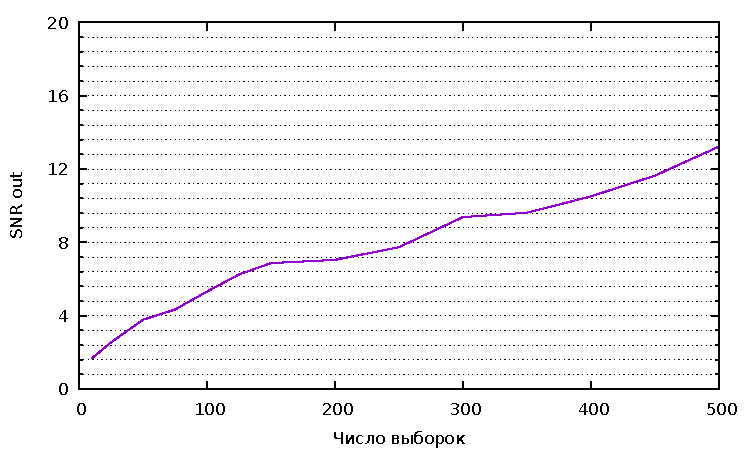
\includegraphics[scale=0.9,page=1]{stat_by_m.pdf}
            \caption{Зависимость SNR от числа циклов накоплений.}
        \end{figure}

    \subsection{Зависимость $\text{SNR}_{\text{out}}$ от $\text{SNR}_{\text{in}}$}
        \begin{table}[H]
            \begin{tabular} { |c|c| }
                \hline
					$\text{SNR}_\text{in}$ & $\text{SNR}_\text{out}$ \\ \hline
                    0.1  &   0.9298	\\ \hline
                    0.2  &   1.7689	\\ \hline
                    0.3  &   2.3864	\\ \hline
                    0.4  &   3.0902	\\ \hline
                    0.5  &   3.6152	\\ \hline
                    0.6  &   5.6947	\\ \hline
                    0.7  &   5.8467	\\ \hline
                    0.8  &   6.6303	\\ \hline
                    0.9  &   7.8079	\\ \hline
                    1    &   8.7068	\\ \hline
                    1.1  &   9.6044	\\ \hline
                    1.2  &   9.7766	\\ \hline
                    1.3  &   11.3096	\\ \hline
                    1.4  &   12.0391	\\ \hline
                    1.5  &   12.8742	\\ \hline
                    1.6  &   13.6251	\\ \hline
                    1.7  &   14.7871	\\ \hline
                    1.8  &   15.1528	\\ \hline
                    1.9  &   15.8292	\\ \hline
                    2    &   16.2992	\\ \hline
            \end{tabular}
            \begin{tabular} { |c|c| }
                \hline
					$\text{SNR}_\text{in}$ & $\text{SNR}_\text{out}$ \\ \hline
                        0.1   &  1.2707	\\ \hline
                        0.2   &  2.5998	\\ \hline
                        0.3   &  4.3951	\\ \hline
                        0.4   &  5.5769	\\ \hline
                        0.5   &  6.8013	\\ \hline
                        0.6   &  7.8619	\\ \hline
                        0.7   &  8.9443	\\ \hline
                        0.8   &  10.7575	\\ \hline
                        0.9   &  12.8911	\\ \hline
                        1     &  13.1404	\\ \hline
                        1.1   &  14.0451	\\ \hline
                        1.2   &  16.08	\\ \hline
                        1.3   &  18.1254	\\ \hline
                        1.4   &  18.5445	\\ \hline
                        1.5   &  21.1901	\\ \hline
                        1.6   &  21.5	\\ \hline
                        1.7   &  22.4446	\\ \hline
                        1.8   &  24.0947	\\ \hline
                        1.9   &  25.0542	\\ \hline
                        2     &  25.6024	\\ \hline
            \end{tabular}
            \begin{tabular} { |c|c| }
                \hline
					$\text{SNR}_\text{in}$ & $\text{SNR}_\text{out}$ \\ \hline
                        0.1  &   1.9678 \\ \hline
                        0.2  &   3.737 \\ \hline
                        0.3  &   5.959 \\ \hline
                        0.4  &   8.4162 \\ \hline
                        0.5  &   9.9779 \\ \hline
                        0.6  &   12.0321 \\ \hline
                        0.7  &   14.0263 \\ \hline
                        0.8  &   15.6813 \\ \hline
                        0.9  &   17.1535 \\ \hline
                        1    &   17.435 \\ \hline
                        1.1  &   21.8457 \\ \hline
                        1.2  &   21.9823 \\ \hline
                        1.3  &   24.8981 \\ \hline
                        1.4  &   24.5258 \\ \hline
                        1.5  &   26.4063 \\ \hline
                        1.6  &   28.4651 \\ \hline
                        1.7  &   30.8562 \\ \hline
                        1.8  &   32.0492 \\ \hline
                        1.9  &   32.2567 \\ \hline
                        2    &   33.5303 \\ \hline
            \end{tabular}
            \caption{Отношение сигнал/шум выхода от сигнал/шум на входе для фиксированного числа выборок (M = 10, 25, 50 соответственно)}
        \end{table}

        \begin{figure}[H]
            \centering
            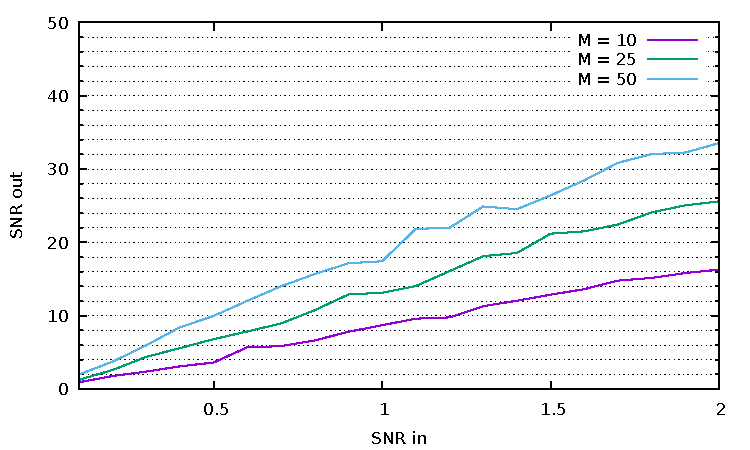
\includegraphics[scale=0.9,page=1]{stat_by_snr.pdf}
            \caption{Зависимость SNR от числа циклов накоплений.}
        \end{figure}

\section{Для квазистационарного сигнала}
    \subsection{Зависимость SNR от числа накоплений}
        \begin{table}[H]
            \centering
            \begin{tabular} { |c|c| }
                \hline
                \textbf{M} & \textbf{SNR} \\ \hline
                    1   &   0.7797  \\ \hline
                    2   &   1.1275  \\ \hline
                    3   &   1.3821  \\ \hline
                    4   &   1.5945  \\ \hline
                    5   &   1.6124  \\ \hline
                    6   &   1.7063  \\ \hline
                    7   &   1.5947  \\ \hline
                    8   &   1.7035  \\ \hline
                    9   &   1.6614  \\ \hline
                    10  &   1.6728  \\ \hline
                    15  &   1.3546  \\ \hline
                    20  &   1.1629  \\ \hline
                    25  &   0.9798  \\ \hline
                    50  &   1.0088  \\ \hline
                    100 &   0.9968  \\ \hline
                    150 &   1.0063  \\ \hline
                    200 &   1.002   \\ \hline
                    250 &   0.998   \\ \hline
                    300 &   1.0092  \\ \hline
                    350 &   1.0017  \\ \hline
                    400 &   0.9916  \\ \hline
                    450 &   1.0034  \\ \hline
                    500 &   0.9981  \\ \hline
            \end{tabular}
            \caption{Отношение сигнал/шум в выходной смеси от длительности накопления}
        \end{table}

        \begin{figure}[H]
            \centering
            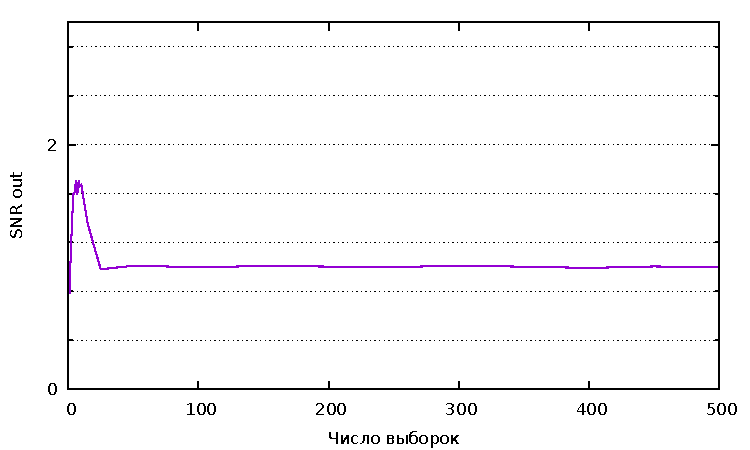
\includegraphics[scale=0.9,page=1]{nonstat_by_m.pdf}
            \caption{Зависимость SNR от числа циклов накоплений.}
        \end{figure}

    \subsection{Зависимость $\text{SNR}_{\text{out}}$ от $\text{SNR}_{\text{in}}$}
        \begin{table}[H]
            \begin{tabular} { |c|c| }
                \hline
					$\text{SNR}_\text{in}$ & $\text{SNR}_\text{out}$ \\ \hline
					0.1i &  1.1005 \\ \hline
					0.2i &  1.6626 \\ \hline
					0.3i &  1.718 \\ \hline
					0.4i &  1.9245 \\ \hline
					0.5i &  2.0495 \\ \hline
					0.6i &  2.2551 \\ \hline
					0.7i &  2.2947 \\ \hline
					0.8i &  2.3052 \\ \hline
					0.9i &  2.3028 \\ \hline
					1  i &  2.3481 \\ \hline
					1.1i &  2.4099 \\ \hline
					1.2i &  2.341 \\ \hline
					1.3i &  2.4444 \\ \hline
					1.4i &  2.4108 \\ \hline
					1.5i &  2.4986 \\ \hline
					1.6i &  2.4083 \\ \hline
					1.7i &  2.4752 \\ \hline
					1.8i &  2.4575 \\ \hline
					1.9i &  2.5077 \\ \hline
					2  i &  2.495 \\ \hline
			\end{tabular}
            \begin{tabular} { |c|c| }
                \hline
					$\text{SNR}_\text{in}$ & $\text{SNR}_\text{out}$ \\ \hline
						0.1 &  0.9702 \\ \hline
						0.2 &  0.9777 \\ \hline
						0.3 &  1.0252 \\ \hline
						0.4 &  1.0131 \\ \hline
						0.5 &  1.0344 \\ \hline
						0.6 &  1.0203 \\ \hline
						0.7 &  1.0157 \\ \hline
						0.8 &  1.0262 \\ \hline
						0.9 &  1.0324 \\ \hline
						1   &  1.0228 \\ \hline
						1.1 &  1.018 \\ \hline
						1.2 &  1.0181 \\ \hline
						1.3 &  1.0198 \\ \hline
						1.4 &  1.0186 \\ \hline
						1.5 &  1.0169 \\ \hline
						1.6 &  1.0254 \\ \hline
						1.7 &  1.0206 \\ \hline
						1.8 &  1.0181 \\ \hline
						1.9 &  1.0208 \\ \hline
						2   &  1.0202 \\ \hline
			\end{tabular}
            \begin{tabular} { |c|c| }
                \hline
					$\text{SNR}_\text{in}$ & $\text{SNR}_\text{out}$ \\ \hline
                            0.1 &  1.0202 \\ \hline
                            0.2 &  0.9996 \\ \hline
                            0.3 &  0.9823 \\ \hline
                            0.4 &  0.9947 \\ \hline
                            0.5 &  0.9909 \\ \hline
                            0.6 &  1.0005 \\ \hline
                            0.7 &  0.9948 \\ \hline
                            0.8 &  1.0087 \\ \hline
                            0.9 &  1.0024 \\ \hline
                            1   &  1.0007 \\ \hline
                            1.1 &  1.0022 \\ \hline
                            1.2 &  1.0017 \\ \hline
                            1.3 &  1.0015 \\ \hline
                            1.4 &  0.9969 \\ \hline
                            1.5 &  0.9993 \\ \hline
                            1.6 &  1.002 \\ \hline
                            1.7 &  0.9993 \\ \hline
                            1.8 &  1.0026 \\ \hline
                            1.9 &  0.9979 \\ \hline
                            2   &  1.0005 \\ \hline
			\end{tabular}
            \caption{Отношение сигнал/шум выхода от сигнал/шум на входе для фиксированного числа выборок (M = 10, 25, 50 соответственно)}
		\end{table}

        \begin{figure}[H]
            \centering
            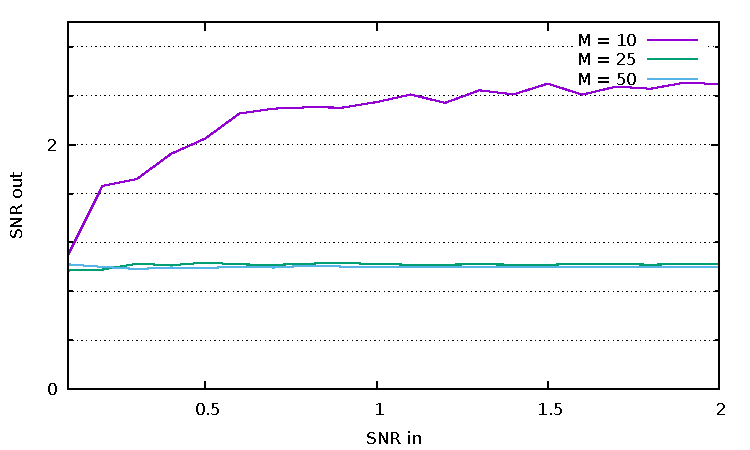
\includegraphics[scale=0.9,page=1]{nonstat_by_snr.pdf}
            \caption{Зависимость SNR от числа циклов накоплений.}
        \end{figure}

\section*{Функциональная схема устройства}
        \begin{figure}[H]
            \centering
            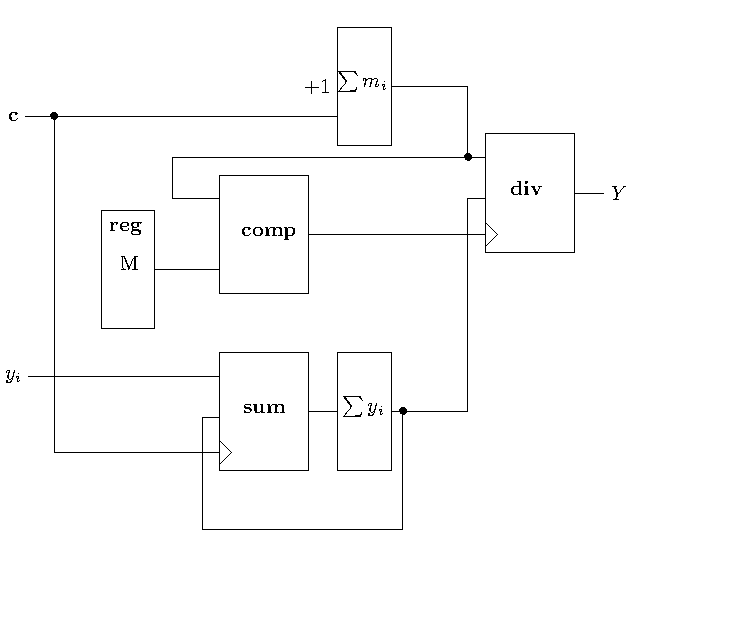
\includegraphics[scale=0.9,page=1]{ffbd.pdf}
        \end{figure}
\section*{Вывод}

\end{document}
